\let\negmedspace\undefined
\let\negthickspace\undefined
\documentclass[journal]{IEEEtran}
\usepackage[a5paper, margin=10mm, onecolumn]{geometry}
%\usepackage{lmodern} % Ensure lmodern is loaded for pdflatex
\usepackage{tfrupee} % Include tfrupee package

\setlength{\headheight}{1cm} % Set the height of the header box
\setlength{\headsep}{0mm}     % Set the distance between the header box and the top of the text

\usepackage{gvv-book}
\usepackage{gvv}
\usepackage{cite}
\usepackage{amsmath,amssymb,amsfonts,amsthm}
\usepackage{algorithmic}
\usepackage{graphicx}
\usepackage{textcomp}
\usepackage{xcolor}
\usepackage{txfonts}
\usepackage{listings}
\usepackage{enumitem}
\usepackage{mathtools}
\usepackage{gensymb}
\usepackage{comment}
\usepackage[breaklinks=true]{hyperref}
\usepackage{tkz-euclide} 
\usepackage{listings}
% \usepackage{gvv}                                        
\def\inputGnumericTable{}                                 
\usepackage[latin1]{inputenc}                                
\usepackage{color}                                            
\usepackage{array}                                            
\usepackage{longtable}                                       
\usepackage{calc}                                             
\usepackage{multirow}                                         
\usepackage{hhline}                                           
\usepackage{ifthen}                                           
\usepackage{lscape}
\begin{document}

\bibliographystyle{IEEEtran}
\vspace{3cm}

\title{12.9.4.13}
\author{EE24BTECH11019 - Dwarak A}
% \maketitle
% \newpage
% \bigskip
{\let\newpage\relax\maketitle}

\renewcommand{\thefigure}{\theenumi}
\renewcommand{\thetable}{\theenumi}
\setlength{\intextsep}{10pt} % Space between text and floats


\numberwithin{equation}{enumi}
\numberwithin{figure}{enumi}
\renewcommand{\thetable}{\theenumi}

\textbf{Question:}\\
Find a particular solution satisfying the differential equation,
\begin{align}
    \cos{\brak{\frac{dy}{dx}}} = a \quad \brak{a\in\mathbb{R}}
\end{align}
given condition,
\begin{align}
    y\brak{0} = 1
    \label{eqn:init_cond}
\end{align}

\solution

\medskip

\textbf{Theoretical Solution:}
\begin{align}
    \frac{dy}{dx} &= \cos^{-1}a \\
    dy &= \brak{\cos^{-1}a}dx
\end{align}

Integration,
\begin{align}
    \int dy &= \int \brak{\cos^{-1}a}dx \\
    y &= \brak{\cos^{-1}a}x + c
    \label{eqn:gen_soln}
\end{align}

To find $c$ substitute \eqref{eqn:init_cond} in \eqref{eqn:gen_soln},
\begin{align}
    1 &= \brak{\cos^{-1}a}\brak{0} + c \\
    1 &= 0 + c \\
    c &= 1
\end{align}

Particular solution,
\begin{align}
    y &= \brak{\cos^{-1}a}x + 1
\end{align}

\medskip

\textbf{Simulated Solution:}

Trapezoidal rule,
\begin{align}
    \int\limits_{x_0}^{x_n}f(x)dx &\approx \frac{h}{2} \brak{f(x_{0}) + 2 \sum_{i=1}^{n-1} f(x_{i}) + f(x_{n}) }
\end{align}

Discretization using trapezoidal rule, integrate $f(x)=cos^{-1}a$ from $x_{n}$ to $x_{n+1}$,
\begin{align}
    y_{n+1}-y_{n} &\approx \frac{h}{2}\brak{f\brak{x_{n}}+f\brak{x_{n+1}}}
\end{align}
    
We can write $f(x_{n+1})$ in terms of $f(x_n)$ using first principle of derivative. $f(x_{n+1})=f(x_n)+hf^{\prime}(x_n)$
\begin{align}
	y_{n+1}-y_{n} &\approx \frac{h}{2}\brak{f\brak{x_{n}}+f\brak{x_{n+1}}} \\
	y_{n+1}-y_{n} &\approx \frac{h}{2}\brak{2f\brak{x_{n}}+hf^\prime\brak{x_{n}}} \\
    y_{n+1} &\approx y_{n} + h\cos^{-1}a + \frac{h^2}{2}(0)
\end{align}

Difference equation,
\begin{align}
    y_{n+1} &\approx y_{n} + h\cos^{-1}a \\
    x_{n+1} &= x_n + h
\end{align}

\begin{figure}[h]
    \centering
    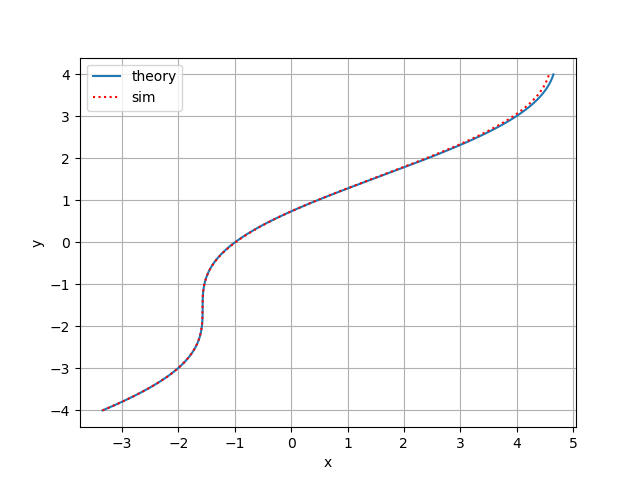
\includegraphics[width=\columnwidth]{figs/plot.png}
    \caption{Plot of the differential equation when $h=0.01$, $a=0.5$}
    \label{fig:Plot1}
    \end{figure}
\end{document}}
